Sketch $\boldsymbol{r}\left(t\right)=\boldsymbol{i}\left(R\sin \omega t +\omega Rt\right)+\boldsymbol{j}\left(R\cos \omega t +R\right)$ taking $R=1$ and $\omega=1$. This curve is called a cycloid and is the path of a point on the rim of a wheel of radius $R$ that rolls without slipping aloing the x-axis. Find the velocity and acceleration at the minimum and maximum y-values of the curve.

The function was plotted in python using a range from 0 to $4\pi$. 
\begin{figure}[h!]
	\centering
	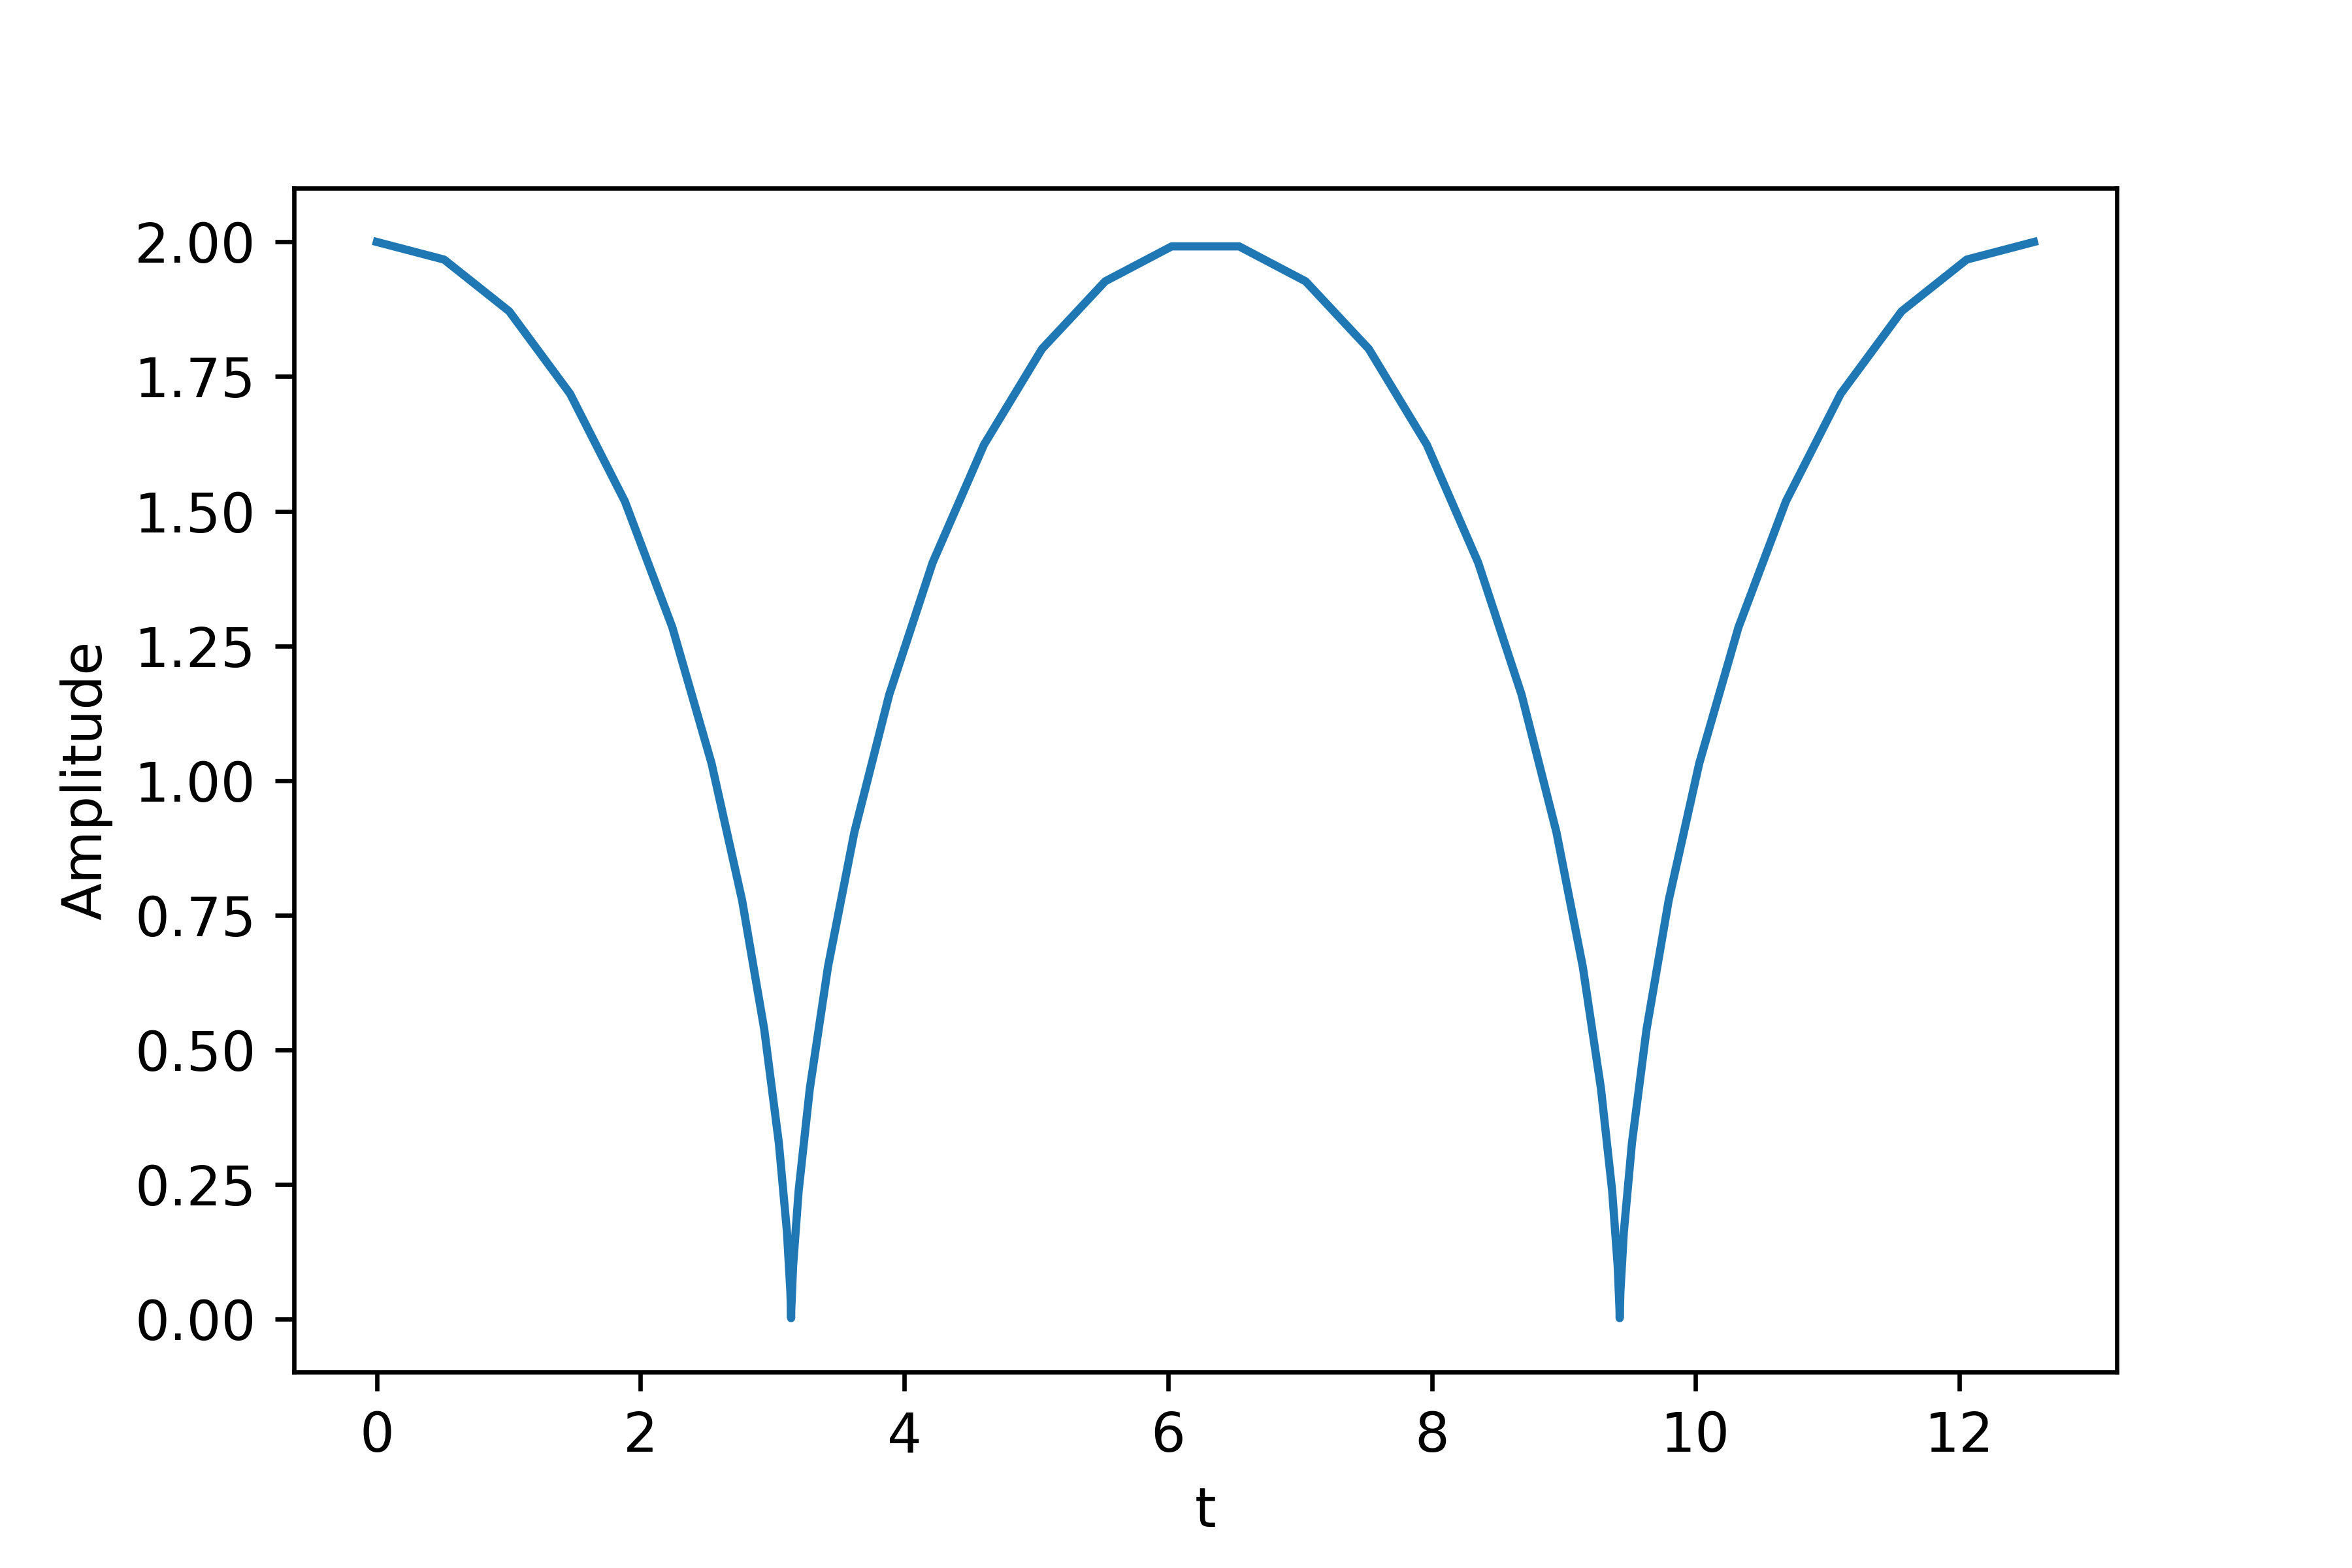
\includegraphics[width=\linewidth]{cycloid.png}
	\caption{Sketch of cycloid with $R=1$ and $\omega=1$.}
\end{figure}

The minimum and maximum y-values are found at $\pi/2$ and 0 respectively.

Velocity is the first derivative and acceleration is the second derivative, equations \ref{eq:vel} and \ref{eq:acc} indicate these respectively.

\begin{equation}
	\boldsymbol{v}=\boldsymbol{r}^\prime=\left(\cos t +1\right)\boldsymbol{i}-\boldsymbol{j}\sin t
	\label{eq:vel}
\end{equation}
\begin{equation}
	\boldsymbol{a}=\boldsymbol{r}^{\prime\prime}=-\boldsymbol{i}\cos t-\boldsymbol{j}\cos t
	\label{eq:acc}
\end{equation}

Evaluation of the velocity at the minimum and maximum result in:
	\begin{equation*}
	\boxed{
			\boldsymbol{v}_{max} =2\boldsymbol{i}
			}
	\end{equation*}
		\begin{equation*}
	\boxed{
		\boldsymbol{v}_{min} = \boldsymbol{i}-\boldsymbol{j}	
			}
	\end{equation*}

\begin{equation*}
	\boxed{
			\boldsymbol{a}_{max}=-\boldsymbol{j}
	}
\end{equation*}
\begin{equation*}
	\boxed{
			\boldsymbol{a}_{min}=-\boldsymbol{i}
	}
\end{equation*}
